\documentclass[10pt]{article}
\usepackage[utf8]{inputenc}\usepackage[T1]{fontenc}\usepackage{lmodern,microtype,booktabs,longtable,tabularx,array,graphicx,xcolor,fancyhdr,xurl}
\usepackage[margin=.82in,headheight=15pt]{geometry}
\definecolor{ink}{HTML}{142B42}\usepackage[colorlinks=true,urlcolor=ink,linkcolor=ink,breaklinks=true]{hyperref}
\hypersetup{pdftitle={Paid Work, Retained Alpha: Evidence and Reproduction Companion}}
\setlength{\parindent}{0pt}\setlength{\parskip}{5pt}\setlength{\emergencystretch}{2em}\renewcommand{\arraystretch}{1.12}
\pagestyle{fancy}\fancyhf{}\fancyhead[L]{Paid Work, Retained Alpha / Evidence}\fancyfoot[C]{\thepage}
\newcommand{\usd}[1]{\$#1}
\begin{document}
\begin{center}{\LARGE\bfseries Evidence and Reproduction Companion}\\[9pt]{\large Profitable Work First. Compounding Capability When Worthwhile.}\\[7pt]27 October 2026 / Evidence cutoff: 26 October 2026\end{center}
\section{Evidence hierarchy}
The simulator and deterministic mechanism were executed locally. Enterprise projects, purchases, collection, frontier reasoning, validation, inventions and investments are simulated. Observed local computation is kept distinct from external reported evidence, arithmetic calibration from sources, and unmeasured behavioral/performance assumptions. No copied benchmark score supplies customer acceptance or demand.
\section{Sources, relevance and limits}


\subsection*{TI-2026 / Transformational Intelligence: Learning to Change the Game}

\textbf{Class:} external reported and analytic. \textbf{Date:} 2026-10.

Operational distinction between purpose, formulation and evaluator; full lifecycle accounting, complementarity and fresh campaign evaluation. Autonomous invention, commercial success or any probability/rate in the new simulation.

\url{https://github.com/MontrealAI/AGI-Alpha-Agent-v0/blob/cb1d232668564fec281dfb0ac834ddbb83ab5115/docs/Transformational_Intelligence.pdf}

\subsection*{ALPHAEVOLVE-2025 / AlphaEvolve: A coding agent for scientific and algorithmic discovery}

\textbf{Class:} external reported. \textbf{Date:} 2025-06-16.

Evaluated code evolution can create useful algorithmic improvements in specified research/engineering environments. Automatic transfer of performance, autonomous intake or profit; no quantitative gain imported.

\url{https://arxiv.org/abs/2506.13131}

\subsection*{ALPHAEVOLVE-CLOUD-2026 / Solve harder problems with AlphaEvolve, now available to everyone on Google Cloud}

\textbf{Class:} external reported. \textbf{Date:} 2026-07-09.

Commercially relevant applications use supplied seed algorithm, background and scoring function before deployment. Independent measurement of reported customer gains; a fully autonomous startup.

\url{https://cloud.google.com/blog/products/ai-machine-learning/alphaevolve-is-available-for-everyone/}

\subsection*{OPTIMUS-2024 / OptiMUS: Scalable Optimization Modeling with (MI)LP Solvers and Large Language Models}

\textbf{Class:} external reported. \textbf{Date:} 2024-02-15.

Task-matched workflow comprising formulation, solver-code construction, debugging and evaluation. Astra/Terra success probabilities, autonomous commercial onboarding or unit costs.

\url{https://arxiv.org/abs/2402.10172}

\subsection*{OPTENGINE-2026 / OPT-Engine: Benchmarking the Limits of LLMs in Optimization Modeling via Complexity Scaling}

\textbf{Class:} external reported. \textbf{Date:} 2026-05-14.

Constraint autoformulation remains a bottleneck under complexity scaling; computation tools do not alone guarantee global constraint compliance. Universal frontier-model ceiling or a numerical performance penalty for this study.

\url{https://arxiv.org/abs/2601.19924v2}

\subsection*{OPTIGUIDE / OptiGuide: GenAI for Supply Chain Optimization}

\textbf{Class:} external reported. \textbf{Date:} undated.

Production what-if support for supply-chain planners is task-relevant feasibility evidence. Removal of planners, unassisted intake, demand or economics.

\url{https://www.microsoft.com/en-us/research/project/optiguide-genai-for-supply-chain-optimization/}

\subsection*{ORTOOLS-ASSIGNMENT / Assignment problems / OR-Tools}

\textbf{Class:} documented capability. \textbf{Date:} undated.

Existing open solver approaches cover assignment problems and should be reused. Algorithm novelty, semantic fidelity of generated customer rules, commercial acceptance.

\url{https://developers.google.com/optimization/assignment/overview}

\subsection*{ORTOOLS-CAPACITY / Assignment with Task Sizes / OR-Tools}

\textbf{Class:} documented capability. \textbf{Date:} undated.

Existing formulation for assigning tasks under resource capacity constraints. General proof for other constraint families.

\url{https://developers.google.com/optimization/assignment/assignment_cp}

\subsection*{NIST-DT-2022 / Credibility Consideration for Digital Twins in Manufacturing}

\textbf{Class:} external reported. \textbf{Date:} 2022-12-16.

Lifecycle verification, validation, uncertainty quantification and intended-use credibility obligations for digital twins. Quantitative automation or engineering-price estimate.

\url{https://www.nist.gov/publications/credibility-consideration-digital-twins-manufacturing}

\subsection*{GSA-4S-2026 / 4S Silversword authorized Federal Supply Schedule price list, contract47QRAA24D0077}

\textbf{Class:} external reported price. \textbf{Date:} 2024-05-01.

Source-backed role-rate anchor for constructed complete-team comparator. Measured effort, actual sale, quotation for this offering, or verified human-only delivery.

Government net labor service schedule, not a package quote. Independent QA charged at engineer rate as a study assumption; broad OR category is imperfectly task matched.

\url{https://www.gsaadvantage.gov/ref_text/47QRAA24D0077/0ZBWRZ.3V29MN_47QRAA24D0077_47QRAA24D0077.PDF}

\subsection*{CLUTCH-2026 / Software Development Company Pricing Guide2026}

\textbf{Class:} external reported price. \textbf{Date:} 2026-09-21.

Cheaper provider stress and geographic range. Matched quote or human-only production.

Broad heterogeneous custom software company services, not matched optimization engagements.

\url{https://clutch.co/developers/pricing}

\subsection*{FEAMAX-2026 / Engineering Project Cost \& Quoting Guide}

\textbf{Class:} external reported price. \textbf{Date:} undated.

Narrow physical-simulation contrast. Full digital twin/invention scope or autonomous professional certification.

Reference ranges subject to geometry, physics, inputs, report and schedule. Software/compute, testing, physical work may be additional; revision terms not fixed.

\url{https://www.feamax.com/cost.html}

\subsection*{BLS-OR-2025 / Operations Research Analysts}

\textbf{Class:} external reported wage. \textbf{Date:} 2026-08.

Employee labor context only. Service price, loaded business cost or contracted team effort.

\url{https://www.bls.gov/ooh/math/operations-research-analysts.htm}

\subsection*{BLS-SWE-QA-2025 / Software Developers, Quality Assurance Analysts, and Testers}

\textbf{Class:} external reported wage. \textbf{Date:} 2026-08.

Employee labor context only. Service price, loaded business cost or contracted team effort.

\url{https://www.bls.gov/ooh/computer-and-information-technology/software-developers.htm}

\subsection*{OAI-01 / GPT-6 Astra model}

Official model specification and tariff. Standard input \$10/M, cached \$1/M, output \$50/M; 1,050,000 context and 128,000 output. Undated alias only in displayed snapshots. Do not infer job-level success, immutable version or user API entitlement. \url{https://developers.openai.com/api/docs/models/gpt-6-astra}

\subsection*{OAI-02 / GPT-6.1 Terra model}

Official model specification and tariff. Standard input \$1/M, cached \$0.05/M, output \$5/M. Tool calling uses Responses API. No claimed equivalence between Pro subscription and API capacity; benchmark suitability is not project accuracy. \url{https://developers.openai.com/api/docs/models/gpt-6.1-terra}

\subsection*{OAI-03 / API pricing}

Web search \$10/1,000 calls plus content tokens; 16GB container \$0.48/20-minute session; indexed file storage \$0.10/GB-day. Eligible containers use minute billing with five-minute minimum. Costs use the conservative full 20-minute unit; storage rate is indexed file storage, not every form of cloud storage. \url{https://developers.openai.com/api/docs/pricing}

\subsection*{OAI-04 / Using GPT-6}

GPT-6 supports Pro execution mode. reasoning.mode=pro aggregates extra model work and bills its tokens at selected-model rates. Some examples still name GPT-5.6. The model slug remains gpt-6-astra; Pro is an execution setting, not unlimited free infrastructure. \url{https://developers.openai.com/api/docs/guides/latest-model}

\subsection*{OAI-05 / GPT-6.1 Terra announcement}

Official launch describes visual reasoning, efficient computer use and writing capability. Reported capabilities motivate execution routing but do not calibrate this workflow or warrant a numerical expert bonus. \url{https://openai.com/index/introducing-gpt-6-1-terra/}

\subsection*{OAI-06 / Reasoning models guide}

Reasoning usage must be budgeted as billed output, including Pro work. Reasoning-token detail is a subset of reported output usage; do not add it twice. \url{https://developers.openai.com/api/docs/guides/reasoning}

\subsection*{PAY-01 / Stripe US standard domestic-card tariff}

Published domestic-card price 2.9\% plus \$0.30 per successful transaction. Illustrative payment-cost comparator, not account availability, authorization, settlement migration or a transaction. \url{https://stripe.com/pricing}

\section{Paid-work and successor foundations}

\subsection*{TI-FOUNDATION / Transformational Intelligence: Learning to Change the Game}

October 2026; 24-page PDF. Full TEX including appendices previously read; all file identities reverified against current repository tree. foundational framework not commercial or frontier performance evidence

Purpose, chosen formulation and evaluator are separate.; A changed representation, information route, dependency or executable protocol must preserve the authorized purpose.; Strong unrestricted alternatives, construction burden, fresh work and falsification remain necessary.

\url{https://github.com/MontrealAI/AGI-Alpha-Agent-v0/blob/d28818dc89a92c40d525d7f0c805e95d8be5978a/docs/Transformational_Intelligence.pdf}\par SHA-256: \nolinkurl{d7170e8217e3bf6aa1b84868c1c76c5994c6995c5297ed092d7e72a6430c664f}.

\url{https://github.com/MontrealAI/AGI-Alpha-Agent-v0/blob/d28818dc89a92c40d525d7f0c805e95d8be5978a/docs/Transformational_Intelligence.tex}\par SHA-256: \nolinkurl{9d4a664d951d6b97f5136bf0b44f1ca458e90d585434a6a27a542694bb2ece5f}.

\subsection*{GYM-SPECIALIST-SUCCESSOR-2.1.0-PRINT / Gym, Specialist ASI \& Successor $\Omega$: The Executable Succession Institution}

v2.1.0, 10 August 2026; 86-page Print PDF. All 86 PDF pages, including full body, appendices, schemas and references, read through text extraction. architectural manuscript with explicit synthetic examples not deployment proof

Separate training/formation knowledge from protected evaluation cases and scorer internals.; Keep negative memory with provenance, scope and validity without turning it into positive capability authority.; Retain mission knowledge, interfaces and evidence while models remain replaceable.; Distinguish environment, candidate, proof, graph admission and consequential action authority.

This manuscript uses Mission Beta for factor sensitivity; the current study uses Beta for the competent moving alternative. These meanings are not equated.; The manuscript proposes lower-confidence-bound admission and institutional authority rules. Those are not imported as extra hurdles or mandatory routine human review.; The named 83-page US Letter v2.1.0 edition is a distinct located file; byte equivalence to this 86-page edition is not asserted.

\url{https://github.com/MontrealAI/MontrealAI.github.io/blob/a9cc143bc05495405ac63b0e2645c425d66410b8/Gym_Specialist_ASI_Successor_Omega_v2_1_0_Print.pdf}\par SHA-256: \nolinkurl{73bad8930e02e5c81e59add0a029c76b3f1b0f9b4f54cf17dfcf2b2768cfb7d8}.

\subsection*{SUCCESSOR-ENTERPRISES-20261022 / Autonomous Enterprises: Activate. Evolve. Scale. --- SUCCESSOR $\Omega$ Harness: Constructing and Financing Reusable Productive Capability}

22 October 2026 source-grounded research manuscript; 27 pages. All 27 PDF pages, including historical corrections, implementation boundaries, appendices and references, read; PDF/TEX matched exact current repository blobs. bounded local construction and source mapping not market or general self improvement evidence

Begin useful bounded work with available capability, then identify recurring burdens and qualify reusable means.; Retain reusable machinery rather than old answers, acceptance decisions, authority or funds.; Preserve the conventional comparator tie, failed transfer and rejected update.; Keep commercial prices, demand, physical validity, model improvement and deployed operation unestablished.

Its Ascension alpha.agent.agi.eth / alpha.club.agi.eth route is historical source context. The new simulated graph uses the user-requested exact direct-label *.agent.agi.eth membership and changes no live route.

\url{https://github.com/MontrealAI/AGI-Alpha-Agent-v0/blob/d28818dc89a92c40d525d7f0c805e95d8be5978a/docs/Autonomous_Enterprises_SUCCESSOR_Omega.pdf}\par SHA-256: \nolinkurl{55aee29b3c8f89bbb2c5002c0874b0cc95dcb144da34f4199184c141bc40ad5f}.

\url{https://github.com/MontrealAI/AGI-Alpha-Agent-v0/blob/d28818dc89a92c40d525d7f0c805e95d8be5978a/docs/Autonomous_Enterprises_SUCCESSOR_Omega.tex}\par SHA-256: \nolinkurl{297407e01609374099f00ca8b758b12c4a5b025c909df8c3181ba7b7d567ea53}.

\subsection*{ALPHA-GUIDED-JOURNEY / Find your Alpha. Build your SUCCESSOR $\Omega$. --- Guided Successor Journey}

. Entire source inspected and copied byte-for-byte. current repository interface documentation not executed four repository deployment

Retain rejected results and earlier cycles without historical resurrection.; Separate discovery, priced unfunded proposal, explicit execution, internal check, external qualification and settlement.; Keep Jobs AGIALPHA and Manager USDC routes distinct.

\url{https://github.com/MontrealAI/AGI-Alpha-Agent-v0/blob/d28818dc89a92c40d525d7f0c805e95d8be5978a/docs/agent/GUIDED_SUCCESSOR_JOURNEY.md}\par SHA-256: \nolinkurl{4b3cb8310a6f025b005c4f3c40d4cb20f3258fa0c685becd65cbe2ce55cb0171}.

\subsection*{ALPHA-REPOSITORY-LICENSE / AGI Alpha Agent repository Apache License 2.0}

.  source license inventory

\url{https://github.com/MontrealAI/AGI-Alpha-Agent-v0/blob/d28818dc89a92c40d525d7f0c805e95d8be5978a/LICENSE}\par SHA-256: \nolinkurl{c71d239df91726fc519c6eb72d318ec65820627232b2f796219e87dcf35d0ab4}.

The 86-page Gym Print manuscript is a read and cited research input. Its all-rights-reserved notice means the raw PDF and extracted text are not redistributed. Its synthetic examples, governance proposals and factor-sensitivity definition of Mission Beta are not substituted for this study's user-defined competent frontier baseline, admission rules or commercial evidence.

\section{Graph drafts, exact provenance and implementation boundary}

\subsection*{GOALOS-V93 / GoalOS V93 --- RSI Validated Skill Graph Ascension Lab}

draft design reference not capability measurement. HTML interface content and all lifecycle JavaScript inspected; no original JavaScript is used to generate study evidence.

Slider-derived proof/utility/canonical scores are not measured performance. Artifact filenames and validator labels are generated templates, not returned work or reviewer evidence. canonicalReview does not require prior Chronicle admission. generateNextMission reads the latest historical Chronicle entry without checking current retirement status. No backend, wallet or actual frontier invocation.

Source SHA-256: \nolinkurl{3c3d606a76ec6a0ca1e854205032042284f83cff866e5eb3f3ae541675dac6ee}.

\url{https://github.com/MontrealAI/MontrealAI.github.io/blob/a9cc143bc05495405ac63b0e2645c425d66410b8/goalos-v93-rsi-validated-skill-graph-ascension-lab-interface.html}

\subsection*{GOALOS-V97.4 / GoalOS V97.4: Private On-Chain Validated Skill Graph}

architecture not deployment or measured performance. Full TEX body read; PDF text extracted and rendered page 5 inspected.

Direct ENS and NameWrapper ownership checks are proposed architecture, not executed in this study. No Ethereum, EIP-712 signature, ZK circuit or production key-management claim. Public ciphertext remains copyable; disclosure/revocation cannot erase authorized plaintext copies.

Source SHA-256: \nolinkurl{ab140a1f7420a6e7c907f4e2f4e51fdb7075ac521b0ffca2bbf59b8e63cbbe2e}.

\url{https://github.com/MontrealAI/goalos-agialpha-sovereign-machine-economy/blob/1e9a5675b1662e98074fb1c71cf2c5b94c7d259f/docs/paper/goalos_private_onchain_zk_vsg.pdf}

\subsection*{GOALOS-V97.4-TEX / GoalOS V97.4 source}

architecture only. 



Source SHA-256: \nolinkurl{435b0a08ed8c1b87d51d986be58264677abf2adaf2d1b41b53063e3b31609898}.

\url{https://github.com/MontrealAI/goalos-agialpha-sovereign-machine-economy/blob/1e9a5675b1662e98074fb1c71cf2c5b94c7d259f/docs/paper/goalos_private_onchain_zk_vsg.tex}

\subsection*{GOALOS-MERKLE-V114 / Merkle Roots for the Validated Skill Graph v114}

commitment foundation not correctness proof. Full source inspected in baseline lane; domain separation, policy binding, state-versus-authority, expiry, revocation and composition sections reviewed again.

Merkle inclusion binds bytes; it does not establish truth, quality, value or authorized current reuse. This lifecycle implementation uses SHA-256 content/event commitments; it does not claim the full typed Merkle forest or on-chain conformance described in the paper.

Source SHA-256: \nolinkurl{3276b66b3aa84d1fadc51d2a398579a8b3108294fafea1a5e239e70dd0fed7de}.

\url{https://github.com/MontrealAI/goalos-agialpha-sovereign-machine-economy/blob/1e9a5675b1662e98074fb1c71cf2c5b94c7d259f/docs/paper/Merkle_Roots_for_the_Validated_Skill_Graph_v114.pdf}

\subsection*{GOALOS-PROOF-LOOPS-V2 / PROOF LOOPS research paper v2 author edition}

process foundation not productive compounding measurement. 

Evidence and admitted capability must be distinguished from work logs or optimistic descriptions. No empirical success or network adoption probability is imported from this source.

Source SHA-256: \nolinkurl{2c41599a893c4c5ac0eacdf9b4416f4420b3d47ee73c04ed868049b29a6055db}.

\url{https://github.com/MontrealAI/goalos-agialpha-sovereign-machine-economy/blob/1e9a5675b1662e98074fb1c71cf2c5b94c7d259f/docs/paper/PROOF_LOOPS_research_paper_v2_author_edition.pdf}

\subsection*{GOALOS-GRAPH-IMAGE / GoalOS Mission Control --- Validated Skill Graph illustration (visible V85 Research Edition)}

visual reference only no calibration. Image visually inspected.

Visible 98.4\% World Class, 99.1\% validated, 2,431 skills, +23.7\% growth and similar dashboard values are illustrative claims, not measurements. No displayed value is used as simulator calibration, evidence of deployed infrastructure, or proof of capability growth.

Located by repository title/path; no supplied attachment fingerprint or original attachment path was available, so exact correspondence is unverified.

Source SHA-256: \nolinkurl{d754fd6f4c79d689ba671f629dfeaae5d8aaf1d4f4e57d84dfe30192176f87d0}.

\url{https://github.com/MontrealAI/MontrealAI.github.io/blob/a9cc143bc05495405ac63b0e2645c425d66410b8/MONTREAL_AI_GoalOS_Bilingual_Institutional_Website_OMEGA_v3_0_0/goalos-assets/img/diagrams/validated-skill-graph.webp}

\subsection*{PYCA-AEAD / PyCA cryptography authenticated encryption documentation}

implementation reference. 

Local AES-GCM verification tests use synthetic payloads and generated ephemeral keys. No production sandbox, endpoint security, ENS identity, chain or ZK verification is tested. The current /latest documentation was development version 51.0.0-dev1 when opened; the installed runtime uses established AESGCM generate\_\allowbreak{}key/encrypt/decrypt methods only.

\url{https://cryptography.io/en/latest/hazmat/primitives/aead/}

The V93 HTML and the V85-labeled dashboard image are preserved as inspected local references with hashes and source links. Their illustrative scores do not calibrate this study. Raw copies without a repository license are not redistributed in the study archive; the new lifecycle implementation is independent. The MIT-licensed GoalOS papers and licenses are preserved. Cryptographic commitments bind bytes, not truth or Alpha.

\section{Component evidence versus projected commercial value}

Initial and recurring assessment units cover bounded synthetic component, version and transfer checks. A reevaluation unit prices a batch of sixteen paired component cases and eight compatibility checks; it does not purchase sixteen complete project pairs. Whole-project acceptance and dollar differences are explicit model extrapolations from component evidence through assumed reliability, demand, scope and collection mappings. These assumptions are stressed, never represented as measured frontier generalization. Prospective graph admission uses remaining incremental retention and reuse costs. Already-accounted-for source-job work is referenced but never charged twice. All job, retention and optional research spending remains in complete enterprise profit.

\section{Human-team scope and effort}

\subsection*{HUMAN-EFFORT-01}

\textbf{evidence class:} explicit\_\allowbreak{}assumption\par

\textbf{scope:} Complete bounded decision-engine engagement with original-rule mapping, runnable API/adapter, baseline, tests, independent QA, deployment package, documentation and up to two bounded revision rounds.\par

\textbf{hours low / or:} 24\par

\textbf{hours low / software:} 40\par

\textbf{hours low / independent qa:} 24\par

\textbf{hours low / systems:} 16\par

\textbf{hours low / pm:} 8\par

\textbf{hours central / or:} 40\par

\textbf{hours central / software:} 80\par

\textbf{hours central / independent qa:} 40\par

\textbf{hours central / systems:} 24\par

\textbf{hours central / pm:} 12\par

\textbf{hours high / or:} 64\par

\textbf{hours high / software:} 120\par

\textbf{hours high / independent qa:} 64\par

\textbf{hours high / systems:} 48\par

\textbf{hours high / pm:} 24\par

\textbf{derived cost usd / low:} 13014.16\par

\textbf{derived cost usd / central:} 22856.28\par

\textbf{derived cost usd / high:} 37174.8\par

\textbf{source rate anchor:} GSA-4S-2026\par

\textbf{limitation:} No matched human trial or authorized comparable quote; workload hours need validation. Not the price of the small mechanistic prototype.\par

\subsection*{MARKET-UNCALIBRATED}

\textbf{evidence class:} unknown\par

\textbf{parameters:} ["buyer willingness to pay", "trust", "adoption", "manual-review willingness", "integration tolerance", "recurrence", "collections"]\par

\textbf{handling:} Use scenarios/thresholds. Neither published provider rates nor technical feasibility calibrate them.\par

\subsection*{FRONTIER-CONSTRUCTION-UNCALIBRATED}

\textbf{evidence class:} unknown\par

\textbf{parameters:} ["autonomous intake and clarification success", "representation construction success", "semantic validation missed errors", "candidate discovery quality", "bundle transfer", "self-acceleration"]\par

\textbf{handling:} Model with transparent distributions and failure controls. External model/solver papers motivate mechanisms, not numeric bonuses.\par

\section{Complete role and stage costs}\begin{table}[htbp]\centering\small
\begin{tabular}{p{.62\linewidth}rr}
\toprule
Activity & USD & Minutes\\\midrule
intake clarification & \usd{5.68} & 60\\
frontier formulation & \usd{67.46} & 360\\
semantic compiler reconstruction & \usd{23.60} & 160\\
task specific compiler adapter & \usd{6.14} & 60\\
solver interface reconstruction & \usd{32.00} & 180\\
project integration & \usd{32.00} & 180\\
independent semantic validation & \usd{31.00} & 180\\
certificate checker reconstruction & \usd{27.80} & 180\\
adversarial harness reconstruction & \usd{9.20} & 90\\
fresh stress and holdout execution & \usd{18.80} & 150\\
packaging handoff & \usd{9.78} & 60\\
\bottomrule\end{tabular}
\caption{Assumed metered usage quantities at official tariffs, per initial complete attempt. Resource minutes are unmeasured workbench occupancy. Construction, retries, storage and overhead are additional.}\end{table}

The initial attempt sums to \usd{263.46}. Each correction costs \usd{37.30} plus \usd{86.80} for revalidation; recovery costs \usd{9.25}. Aggregated billed tokens include Pro subwork and reasoning. They are spread across multiple requests; no free cache or subscription allowance is deducted.
\begin{table}[htbp]\centering\small\begin{tabular}{lrrr}
\toprule
Retention option & Extra USD & Workbench min. & Billed tokens (M)\\\midrule
R & \usd{290.05} & 2,430 & 16.26\\
V & \usd{307.95} & 2,550 & 16.78\\
bundle & \usd{569.72} & 4,770 & 30.15\\
\bottomrule\end{tabular}\caption{Primary ledger B: additional one-domain extraction, generalization, fresh validation and portable packaging. Source-job construction remains in ledger A and is not charged again. Candidate scans, later reuse and upkeep are additional.}\end{table}

A paid candidate scan costs \usd{3.12}, including scans that find no useful skill. An optimistic direct-cost-only screen requires 5.2 compatible R uses, 8.3 V uses, or 6.2 joint uses. These bounds exclude acquisition, failed extraction, overlap, ongoing checks, maintenance, erosion and delay. They are not observed demand or guaranteed repayment.
\begin{table}[htbp]\centering\small\begin{tabular}{lrrr}
\toprule
Separate campaign & USD & Workbench min. & Billed tokens (M)\\\midrule
R & \usd{5,959.60} & 43,440 & 368.56\\
V & \usd{8,764.00} & 67,440 & 510.56\\
bundle & \usd{13,334.00} & 101,760 & 770.84\\
\bottomrule\end{tabular}\caption{Optional ledger C: deliberate separate research, not a mandatory fee per job-born skill. All attempts and construction are charged once. These broader campaigns are distinct from the primary domain-specific retention options.}\end{table}

For optional separate research, an optimistic reconstruction-only screen requires 107.2 compatible uses for R, 236.9 for V and 144.0 for the bundle. These are different activities and scopes from the primary job-born capsules. They omit failed construction, acquisition, overlap, maintenance, obsolescence and delay. This calculation cannot establish demand.
\begin{table}[htbp]\centering\small\begin{tabular}{p{.62\linewidth}rr}
\toprule
Network activity & USD / unit & Workbench min.\\\midrule
network access & \usd{1.45} & 15\\
network distribution & \usd{0.73} & 10\\
recipient acquisition & \usd{8.39} & 90\\
network composition & \usd{4.17} & 60\\
asset maintenance month & \usd{7.02} & 60\\
asset revalidation unit & \usd{19.20} & 120\\
beta version reevaluation & \usd{48.00} & 480\\
graph revocation propagation & \usd{1.05} & 15\\
\bottomrule\end{tabular}\caption{Additional network lifecycle work. Quantities and small non-model allowances are assumptions, priced using the same official tariffs. The simulator states the triggering event and frequency; these are not observed graph-service fees.}\end{table}


\subsection*{intake clarification}

Automated scope negotiation, schema checks, clarification, safe non-safety-critical boundary, and buyer-provided constraint confirmation.

Astra billed input/output: 240,000 / 40,000. Terra: 400,000 / 40,000. Container sessions: 1. Other tools: \usd{0.20}. Derived cost: \usd{5.68}. All quantities are assumptions.

\subsection*{frontier formulation}

Astra Pro reasons over the new domain, objectives, constraints, alternatives and acceptance evidence. New-job reasoning is retained in full.

Astra billed input/output: 3,000,000 / 600,000. Terra: 500,000 / 80,000. Container sessions: 12. Other tools: \usd{0.80}. Derived cost: \usd{67.46}. All quantities are assumptions.

\subsection*{semantic compiler reconstruction}

Reconstruct the reusable DSL parser, typed constraint lowering and compiler core when the recipient lacks an equivalent admitted asset.

Astra billed input/output: 800,000 / 160,000. Terra: 400,000 / 64,000. Container sessions: 14. Other tools: \usd{0.16}. Derived cost: \usd{23.60}. All quantities are assumptions.

\subsection*{task specific compiler adapter}

Create and verify the new buyer-specific mapping and adapter, even when the compiler core is reused.

Astra billed input/output: 200,000 / 40,000. Terra: 100,000 / 16,000. Container sessions: 4. Other tools: \usd{0.04}. Derived cost: \usd{6.14}. All quantities are assumptions.

\subsection*{solver interface reconstruction}

Reconstruct the reusable solver adapter, executable API and packaging scaffold; the underlying public optimization algorithm is not claimed as a new discovery.

Astra billed input/output: 800,000 / 120,000. Terra: 2,000,000 / 300,000. Container sessions: 30. Other tools: \usd{0.10}. Derived cost: \usd{32.00}. All quantities are assumptions.

\subsection*{project integration}

Integrate new task data, configuration, API contracts and executable handoff; automated execution is charged even with retained assets.

Astra billed input/output: 800,000 / 120,000. Terra: 2,000,000 / 300,000. Container sessions: 30. Other tools: \usd{0.10}. Derived cost: \usd{32.00}. All quantities are assumptions.

\subsection*{independent semantic validation}

Astra Pro independently checks the original buyer constraints, objective and scope; Terra executes evidence checks. Shared specification error remains possible.

Astra billed input/output: 1,000,000 / 200,000. Terra: 800,000 / 80,000. Container sessions: 20. Other tools: \usd{0.20}. Derived cost: \usd{31.00}. All quantities are assumptions.

\subsection*{certificate checker reconstruction}

Reconstruct the residual-certificate checker, original-capacity checks and counterexample localization when no equivalent verifier asset exists.

Astra billed input/output: 600,000 / 120,000. Terra: 800,000 / 100,000. Container sessions: 30. Other tools: \usd{0.10}. Derived cost: \usd{27.80}. All quantities are assumptions.

\subsection*{adversarial harness reconstruction}

Reconstruct the reusable mutation/property/stress-test harness. Reuse avoids harness construction, not fresh test execution.

Astra billed input/output: 200,000 / 40,000. Terra: 200,000 / 30,000. Container sessions: 10. Other tools: \usd{0.05}. Derived cost: \usd{9.20}. All quantities are assumptions.

\subsection*{fresh stress and holdout execution}

Generate and execute fresh cases, held-out tests, fault injection and failure analysis under the new project specification.

Astra billed input/output: 200,000 / 40,000. Terra: 200,000 / 30,000. Container sessions: 30. Other tools: \usd{0.05}. Derived cost: \usd{18.80}. All quantities are assumptions.

\subsection*{packaging handoff}

Generate reproducible package, evidence manifest, scope limitations, API instructions and automated buyer handoff.

Astra billed input/output: 320,000 / 48,000. Terra: 800,000 / 80,000. Container sessions: 6. Other tools: \usd{0.10}. Derived cost: \usd{9.78}. All quantities are assumptions.

\subsection*{correction}

Astra Pro diagnoses the failed evidence and designs a repair; Terra implements and executes it. Full revalidation is charged separately.

Astra billed input/output: 800,000 / 160,000. Terra: 1,200,000 / 160,000. Container sessions: 40. Other tools: \usd{0.10}. Derived cost: \usd{37.30}. All quantities are assumptions.

\subsection*{revalidation}

Full independent semantic/certificate/adversarial revalidation after correction; no assumed free validator.

Astra billed input/output: 2,000,000 / 400,000. Terra: 2,000,000 / 240,000. Container sessions: 90. Other tools: \usd{0.40}. Derived cost: \usd{86.80}. All quantities are assumptions.

\subsection*{recovery}

Bounded automated environment/tool recovery; repeated failure ends in paid abstention or rejection, not a hidden human team.

Astra billed input/output: 160,000 / 32,000. Terra: 800,000 / 80,000. Container sessions: 10. Other tools: \usd{0.05}. Derived cost: \usd{9.25}. All quantities are assumptions.

\subsection*{asset construction unit}

One candidate reusable capability construction/research attempt, including unsuccessful attempts.

Astra billed input/output: 6,000,000 / 1,200,000. Terra: 6,000,000 / 800,000. Container sessions: 180. Other tools: \usd{2.00}. Derived cost: \usd{218.40}. All quantities are assumptions.

\subsection*{asset evaluation unit}

One independent Astra Pro component-evaluation bundle plus fresh execution and adversarial tests for a capability candidate. Campaign counts cover candidate screening, unsuccessful attempts and a final held-out component/transfer suite; they are not complete buyer-project pairs.

Astra billed input/output: 4,000,000 / 800,000. Terra: 4,000,000 / 400,000. Container sessions: 240. Other tools: \usd{0.50}. Derived cost: \usd{201.70}. All quantities are assumptions.

\subsection*{asset integration unit}

Capability versioning, typed dependency and scope integration, graph-admission evidence, and packaging.

Astra billed input/output: 480,000 / 80,000. Terra: 2,000,000 / 200,000. Container sessions: 30. Other tools: \usd{0.10}. Derived cost: \usd{26.30}. All quantities are assumptions.

\subsection*{paid job emergence scan}

Inspect an observed validator-approved commercial-delivery artifact and its charged usage receipts for a reusable candidate, recipient gap, scope and dependencies. Payment authorization and actual collection are recorded separately; this scan cannot observe latent true correctness or future collections. A scan may find nothing and is charged once when invoked.

Astra billed input/output: 100,000 / 20,000. Terra: 100,000 / 10,000. Container sessions: 2. Other tools: \usd{0.00}. Derived cost: \usd{3.12}. All quantities are assumptions.

\subsection*{incremental artifact extraction}

Extract the already-built commercial-job artifact and its evidence/provenance into a candidate envelope. The original compiler, solver, checker or stress construction has already been charged to its originating job and is not billed again, whether or not the customer has yet paid.

Astra billed input/output: 180,000 / 36,000. Terra: 400,000 / 40,000. Container sessions: 4. Other tools: \usd{0.02}. Derived cost: \usd{6.15}. All quantities are assumptions.

\subsection*{incremental generalization R}

Additional work only: remove buyer-specific constants from the existing compiler/solver artifact, parameterize supported schema differences, define typed interfaces and bounded recipient compatibility. Original paid-job construction remains allocated to its originating job.

Astra billed input/output: 1,200,000 / 240,000. Terra: 2,000,000 / 200,000. Container sessions: 60. Other tools: \usd{0.10}. Derived cost: \usd{55.90}. All quantities are assumptions.

\subsection*{incremental generalization V}

Additional work only: generalize the existing certificate/checker and counterexample harness across supported schema variants, isolate original-constraint tests and create reusable test adapters. The original paid-job checker/harness remains charged solely to its job.

Astra billed input/output: 1,600,000 / 320,000. Terra: 2,000,000 / 240,000. Container sessions: 80. Other tools: \usd{0.20}. Derived cost: \usd{73.80}. All quantities are assumptions.

\subsection*{network access}

Read current graph and Beta-version metadata; check simulated eligibility, signature structure, membership and scope before any acquisition. Paid even when an equivalent capability is already available. No token-price revenue is credited.

Astra billed input/output: 40,000 / 8,000. Terra: 100,000 / 10,000. Container sessions: 1. Other tools: \usd{0.00}. Derived cost: \usd{1.45}. All quantities are assumptions.

\subsection*{network distribution}

Deliver one versioned artifact and evidence package to one authorized simulated recipient; verify content hashes and receipt. Transport/storage allowance is an assumption, not a published AGIALPHA fee.

Astra billed input/output: 0 / 0. Terra: 100,000 / 10,000. Container sessions: 1. Other tools: \usd{0.00}. Derived cost: \usd{0.73}. All quantities are assumptions.

\subsection*{recipient acquisition}

Recipient capability-gap check, scope adaptation, admission test and integration; no benefit for an existing equivalent recipient.

Astra billed input/output: 200,000 / 32,000. Terra: 500,000 / 80,000. Container sessions: 8. Other tools: \usd{0.05}. Derived cost: \usd{8.39}. All quantities are assumptions.

\subsection*{network composition}

Additional cross-asset dependency/interface/composition checks for a genuinely composed use; individual recipient integration and fresh job semantic validation remain distinct.

Astra billed input/output: 80,000 / 16,000. Terra: 400,000 / 40,000. Container sessions: 4. Other tools: \usd{0.00}. Derived cost: \usd{4.17}. All quantities are assumptions.

\subsection*{asset maintenance month}

Automatic monthly monitoring, dependency refresh and bounded maintenance per active asset.

Astra billed input/output: 200,000 / 40,000. Terra: 400,000 / 40,000. Container sessions: 5. Other tools: \usd{0.02}. Derived cost: \usd{7.02}. All quantities are assumptions.

\subsection*{asset revalidation unit}

Fresh version/freshness/revocation/composition revalidation for a retained capability.

Astra billed input/output: 400,000 / 80,000. Terra: 1,000,000 / 100,000. Container sessions: 20. Other tools: \usd{0.10}. Derived cost: \usd{19.20}. All quantities are assumptions.

\subsection*{beta version reevaluation}

One fresh component/version reevaluation batch: 16 paired bounded component-oracle cases plus 8 scoped recipient-transfer checks, within the declared 480 critical-workbench minutes and 60 container sessions. This is not 16 paired complete buyer projects. Full-project acceptance, collections and net value are conditional model extrapolations from component observations and separate commercial assumptions.

Astra billed input/output: 800,000 / 160,000. Terra: 2,000,000 / 200,000. Container sessions: 60. Other tools: \usd{0.10}. Derived cost: \usd{48.00}. All quantities are assumptions.

\subsection*{graph revocation propagation}

Propagate one revocation/freshness/dependency invalidation to one recipient and prevent further admitted use; refresh the local evidence state. Authentication in the study is simulated.

Astra billed input/output: 20,000 / 4,000. Terra: 100,000 / 10,000. Container sessions: 1. Other tools: \usd{0.00}. Derived cost: \usd{1.05}. All quantities are assumptions.

\section{Executed local mechanism and independent QA}

The frozen synthetic mechanism run used 120 exhaustive small comparisons and 180 larger instances. All 300 passed their original-model checks. The unrestricted rebuild matched every output. The supplied problem family and candidate were researcher designed. Semantic truth, autonomous invention and commercial suitability were not measured.

Mutation and negative controls cover objectives, capacities, eligibility, suboptimal assignments, unsupported rules and infeasibility. A shared wrong model passes its own checker. Local median producer/checker times are 0.0776 / 0.0913 ms; these exclude model/API work and are not throughput calibration.

An additional independent QA program enumerated 6,727 assignments across 96 cases and found no mismatch between checker acceptance and actual feasible optimality. This post-protocol QA is not pooled into the 300 primary mechanism instances.

\clearpage\section{Frozen economic parameter register}

Entries below reproduce the executed configuration. Except source tariffs and derived arithmetic, these are explicit assumptions or policy choices. A probability in this table is not an empirical confidence interval. The code and complete machine-readable configuration control exact behavior.

\subsection*{study id}

"PAID-WORK-RETAINED-ALPHA-2026-10-26-v3"

\subsection*{status}

"Prespecified paid-job-learning study; parameters freeze before independent confirmation."

\subsection*{currency}

"USD, pre-tax; transaction-tax pass-through and corporate-income-tax schedules excluded"

\subsection*{train seed}

951043

\subsection*{test seed}

951251

\subsection*{months}

24

\subsection*{runoff months}

3

\subsection*{seed cash}

20000

\subsection*{discovery cost}

5250.6

\subsection*{discovery budget counts}

\begin{longtable}{p{.44\linewidth}p{.50\linewidth}}\toprule Parameter & Value \\\midrule\endhead

asset construction unit & 12\\

asset evaluation unit & 8\\

asset integration unit & 30\\

intake clarification & 40\\

\bottomrule\end{longtable}

\subsection*{cost register}

"../evidence/workflow\_\allowbreak{}costs\_\allowbreak{}v3.json"

\subsection*{human reference}

\begin{longtable}{p{.44\linewidth}p{.50\linewidth}}\toprule Parameter & Value \\\midrule\endhead

central & 22856\\

low & 13014\\

high & 37175\\

basis & Published GSA role rates multiplied by explicit assumed multidisciplinary effort; not a received quote or proof of human-only methods.\\

\bottomrule\end{longtable}

\subsection*{price fractions}

[0.2, 0.25, 0.3, 0.35, 0.4, 0.45, 0.5, 0.55, 0.6, 0.65, 0.7, 0.75, 0.8, 0.85, 0.9, 0.95, 1.0, 1.05, 1.1, 1.15, 1.2]

\subsection*{fixed price ablation}

0.65

\subsection*{operations}

\begin{longtable}{p{.44\linewidth}p{.50\linewidth}}\toprule Parameter & Value \\\midrule\endhead

monthly control cost & 200\\

monthly business automation cost & 300\\

monthly workbench minutes & 46080\\

monthly token quota & 500000000\\

research fraction limit & 0.7\\

reserve months & 3\\

warranty reserve fraction & 0.06\\

payment fraction & 0.029\\

payment fixed & 0.3\\

storage per delivery & 3\\

max queue age months & 1\\

max corrections & 2\\

postdelivery discovery & 0.8\\

admission abstention & 0.06\\

monthly common burst probability & 0.06\\

burst capacity multiplier & 0.65\\

burst semantic penalty & 0.12\\

burst shared error increment & 0.06\\

routine provider human minutes & 0\\

qualification units per opportunity & 2\\

collection timing & collection\_\allowbreak{}probability is observed payment authorization at delivery. Authorized amounts settle after collection\_\allowbreak{}lag months; no later counterparty default is modeled. Failed authorization is known at delivery and incurs all work costs. Only cleared cash may fund spending.\\

fixed automation scope & Monthly control and business-automation fees cover deterministic monitoring, billing/listings and orchestration subscriptions, not unmetered frontier-model calls.\\

\bottomrule\end{longtable}

\subsection*{market}

\begin{longtable}{p{.44\linewidth}p{.50\linewidth}}\toprule Parameter & Value \\\midrule\endhead

value grid & [0.9, 1.3, 1.8]\\

trust grid & [0.04, 0.14, 0.3]\\

prior weights & [1, 1, 1, 1, 1, 1, 1, 1, 1]\\

value log sigma & 0.3\\

taste scale fraction & 0.12\\

human quality belief & 0.96\\

our quality belief & 0.9\\

human review fraction & 0.04\\

our review fraction & 0.06\\

integration fraction & 0.08\\

postpone utility fraction & 0.02\\

arrival prior shape & 2\\

arrival prior rate & 0.5\\

observed choice & Only our purchase/nonpurchase; other choices are analyst-only latent labels.\\

price game & Seller posts a bounded-grid price; buyers best respond among our package, human service, retain current method and decline. Outside-provider prices are exogenous in primary; no Nash claim.\\

base delivery days & 5\\

human delivery days & 5\\

delay cost fraction per day & 0.002\\

switching fraction within integration & 0.03\\

observed incident trust coefficient & 1.0\\

\bottomrule\end{longtable}

\subsection*{scope}

\begin{longtable}{p{.44\linewidth}p{.50\linewidth}}\toprule Parameter & Value \\\midrule\endhead

domains & 6\\

recipient agents & 12\\

base share & 0.7\\

rich human reference multiplier & 1.6\\

rich activity multiplier & 1.8\\

supported domain fraction & 0.85\\

partial reconstruction saving & 0.35\\

existing equivalent R & 0.25\\

existing equivalent V & 0.2\\

partial equivalent probability & 0.25\\

ordinary case specific learning probability & 0.06\\

sampling unit & A distinct buyer/deployment or genuinely new integration/schema contract producing the full executable decision-engine package. Repeated allocation answers or changing cost/capacity/eligibility inputs inside a sold engine are included and create no additional full-package sale.\\

domain names & ["new\_\allowbreak{}capacity\_\allowbreak{}schema\_\allowbreak{}deployment", "new\_\allowbreak{}eligibility\_\allowbreak{}schema\_\allowbreak{}deployment", "new\_\allowbreak{}cost\_\allowbreak{}model\_\allowbreak{}deployment", "new\_\allowbreak{}source\_\allowbreak{}adapter\_\allowbreak{}deployment", "new\_\allowbreak{}compound\_\allowbreak{}schema\_\allowbreak{}deployment", "unsupported\_\allowbreak{}nonlinear\_\allowbreak{}extension"]\\

ordinary case specific learning description & Observed approved deliveries may leave narrow setup/context metadata. This reduces a small fraction of later reconstruction activity but never increases mechanical or semantic correctness; it does not create a broad admitted component or free transfer.\\

domain weights & [0.23, 0.2, 0.2, 0.19, 0.18]\\

domain semantic penalties & [0, 0.02, 0.03, 0.04, 0.06, 0]\\

recipient specialties & [[0, 1], [1, 2], [2, 3], [3, 4], [4, 0], [0, 1], [1, 2], [2, 3], [3, 4], [4, 0], [0, 1], [1, 2]]\\

specialist routing fraction & 0.7\\

\bottomrule\end{longtable}

\subsection*{assets}

\begin{longtable}{p{.44\linewidth}p{.50\linewidth}}\toprule Parameter & Value \\\midrule\endhead

R / bit & 1\\

R / campaign & R\\

R / domains & [0, 1, 2, 3, 4]\\

R / lifetime months & 18\\

R / obsolescence probability & 0.02\\

R / pilot cases & 24\\

R / pilot pass threshold & 0.9\\

V / bit & 2\\

V / campaign & V\\

V / domains & [0, 1, 2, 3, 4]\\

V / lifetime months & 18\\

V / obsolescence probability & 0.02\\

V / pilot cases & 24\\

V / pilot pass threshold & 0.9\\

\bottomrule\end{longtable}

\subsection*{policy}

\begin{longtable}{p{.44\linewidth}p{.50\linewidth}}\toprule Parameter & Value \\\midrule\endhead

forecast months & 18\\

value hurdle fraction & 0\\

minimum research cash headroom & 1000\\

financial monthly discount rate & 0.005\\

allow seed funded research & True\\

pilot only observable & True\\

exploration & None in primary price controller; Bayesian learning uses endogenous purchased/nonpurchased offers. Optional exploration is a separate ablation.\\

objective & Approximate posterior expected terminal pre-tax cash net of seed; receding-horizon one-campaign lookahead, not globally optimal POMDP. Cash/reserve and conservative next-period solvency constraints are separate eligibility constraints.\\

risk constraint & Deterministic protection of known liabilities, reserve-month fixed obligations and cash headroom; no claim of a general probabilistic cash-shortfall guarantee. Monte Carlo insolvency is reported separately.\\

\bottomrule\end{longtable}

\subsection*{scenarios}

\begin{longtable}{p{.44\linewidth}p{.50\linewidth}}\toprule Parameter & Value \\\midrule\endhead

conservative / human reference & 13014\\

conservative / arrivals month & 1\\

conservative / arrival growth & 0\\

conservative / world arrival log sigma & 0.45\\

conservative / buyer value multiplier & 0.9\\

conservative / buyer trust fraction & 0.3\\

conservative / semantic correctness & 0.68\\

conservative / reconstruction correctness & 0.84\\

conservative / retained component correctness & 0.96\\

conservative / semantic validator sensitivity & 0.75\\

conservative / mechanical validator sensitivity & 0.94\\

conservative / validator specificity & 0.97\\

conservative / shared fault probability & 0.1\\

conservative / shared fault miss & 0.4\\

conservative / correction success & 0.45\\

conservative / collection probability & 0.9\\

conservative / collection lag & 2\\

conservative / asset build success & 0.65\\

conservative / transfer success & 0.65\\

conservative / activity quantity multiplier & 1.5\\

central / human reference & 22856\\

central / arrivals month & 4\\

central / arrival growth & 0.01\\

central / world arrival log sigma & 0.35\\

central / buyer value multiplier & 1.3\\

central / buyer trust fraction & 0.14\\

central / semantic correctness & 0.85\\

central / reconstruction correctness & 0.93\\

central / retained component correctness & 0.985\\

central / semantic validator sensitivity & 0.88\\

central / mechanical validator sensitivity & 0.98\\

central / validator specificity & 0.98\\

central / shared fault probability & 0.05\\

central / shared fault miss & 0.25\\

central / correction success & 0.68\\

central / collection probability & 0.96\\

central / collection lag & 1\\

central / asset build success & 0.8\\

central / transfer success & 0.82\\

central / activity quantity multiplier & 1.0\\

favorable / human reference & 37175\\

favorable / arrivals month & 8\\

favorable / arrival growth & 0.02\\

favorable / world arrival log sigma & 0.25\\

favorable / buyer value multiplier & 1.8\\

favorable / buyer trust fraction & 0.04\\

favorable / semantic correctness & 0.94\\

favorable / reconstruction correctness & 0.97\\

favorable / retained component correctness & 0.995\\

favorable / semantic validator sensitivity & 0.95\\

favorable / mechanical validator sensitivity & 0.995\\

favorable / validator specificity & 0.99\\

favorable / shared fault probability & 0.02\\

favorable / shared fault miss & 0.12\\

favorable / correction success & 0.82\\

favorable / collection probability & 0.99\\

favorable / collection lag & 1\\

favorable / asset build success & 0.9\\

favorable / transfer success & 0.92\\

favorable / activity quantity multiplier & 0.8\\

\bottomrule\end{longtable}

\subsection*{nonclaims}

["No novel optimization algorithm is claimed.", "Synthetic mechanism correctness does not calibrate frontier model accuracy.", "No real buyers, provider model execution, transactions or ENS authentication are represented as observed.", "No prescribed price discount or minimum number of investments defines success.", "Missing retained assets do not remove the frontier baseline's ability to reconstruct the same compiler and checker.", "Candidate, validated artifact, admitted positive expected Alpha and realized net value are distinct.", "Moving Beta schedules and modeled net-Alpha estimates are assumptions, not observed autonomous invention or a permanent moat.", "Shared versus private network policies have identical agent counts and aggregate provider quotas."]

\subsection*{network}

\begin{longtable}{p{.44\linewidth}p{.50\linewidth}}\toprule Parameter & Value \\\midrule\endhead

creator recipient & 0\\

admission mean gain prior & 0.0\\

admission prior effective cases & 8\\

assessment minimum cases & 12\\

scope & Authenticated direct-label *.agent.agi.eth members; simulated identity checks only. All shareable admitted Alpha is discoverable and optionally usable by every member subject to scope, versions, prerequisites, freshness and revocation. No club authority changes.\\

beta epochs & [\{"month": 1, "version": "beta-1", "reconstruction\_\allowbreak{}quantity\_\allowbreak{}factor": 1.0, "public\_\allowbreak{}equivalent\_\allowbreak{}probability\_\allowbreak{}per\_\allowbreak{}month": 0.015\}, \{"month": 9, "version": "beta-2", "reconstruction\_\allowbreak{}quantity\_\allowbreak{}factor": 0.8, "public\_\allowbreak{}equivalent\_\allowbreak{}probability\_\allowbreak{}per\_\allowbreak{}month": 0.05\}, \{"month": 17, "version": "beta-3", "reconstruction\_\allowbreak{}quantity\_\allowbreak{}factor": 0.65, "public\_\allowbreak{}equivalent\_\allowbreak{}probability\_\allowbreak{}per\_\allowbreak{}month": 0.08\}]\\

alpha forecast horizon months & 12\\

reassessment cases & 16\\

retirement if nonpositive & True\\

fixed compute comparison & True\\

initial beta description & Competent current frontier models, public optimization tools and every already available recipient-compatible retained or equivalent capability; no absence-of-file incapability assumption.\\

evidence max age months & 4\\

periodic reassessment months & 3\\

alpha activity effect fraction & 1.0\\

alpha quality effect fraction & 1.0\\

effect interpretation & Named reconstructible activities are avoided only after supported admission and successful recipient adaptation. Fractions expose uncertain transfer of component activity/reliability into complete project work; they are not a generic expert-use bonus.\\

\bottomrule\end{longtable}

\subsection*{paid job learning}

\begin{longtable}{p{.44\linewidth}p{.50\linewidth}}\toprule Parameter & Value \\\midrule\endhead

enabled & True\\

scan probability & 0.35\\

candidate probability given scan & 0.25\\

rights available probability & 0.95\\

retention generalization success & 0.85\\

primary scope domains & 1\\

optional research enabled & True\\

local artifact reuse in beta & True\\

candidate trigger & Observable validated delivery, irrespective of latent material correctness or future collections. Source rights and portability are simulated and may fail.\\

scope boundary & One source-job-bound schema capsule. No global capability emerges from one bespoke job. Original installed-engine uses remain included and are never new full-package sales.\\

local reuse boundary & The originator retains ordinary useful source artifacts in its competent Beta. Paid Alpha retention pays only incremental sanitized portability/generalization and new evidence.\\

assessment strata & ["dense\_\allowbreak{}standard", "sparse\_\allowbreak{}eligibility", "tight\_\allowbreak{}capacity", "ties\_\allowbreak{}and\_\allowbreak{}degeneracy"]\\

free ordinary reuse across agents & False\\

\bottomrule\end{longtable}

\section{Results, audit and reproduction}

All 18 adversarial lifecycle cases passed. The replay contains 229 recorded steps, including 53 rejected operations; these are software test actions, not independent invention campaigns or commercial projects. The publication builder independently verifies 227 event commitments and the exact implementation/test hashes before presenting them. The implementation SHA-256 is \nolinkurl{ea7808682a0b8cddfa7f246db3abcb3faff3e68dae3fc6a6e9ae21480f0ed40f}.
\begin{table}[htbp]\centering\small\begin{tabular}{p{.25\linewidth}p{.68\linewidth}}
\toprule
Test family & Executed boundary\\\midrule
Admission and value & Prospective incremental Alpha; source-job receipts are not charged twice; duplicate and negative-value candidates rejected.\\
Authority and freshness & Exact direct names; distinct roles; stale evidence, Beta/policy/registry changes and immutable public views.\\
History and composition & Canonical bypass blocked; revocation and retirement survive old history; dependencies checked transitively.\\
Privacy and actions & AES-GCM tampering, trusted executors, explicit action permission, export controls and protected evaluation/scorer exclusion.\\
History and learning & Separate failure memory cannot enter positive discovery; origin records bind observable delivery and receipt provenance.\\
\bottomrule\end{tabular}\caption{Research implementation tests. Synthetic identities and economic assessments are not real validators or operational capability evidence.}\end{table}
The export test deliberately retains previously authorized plaintext after revocation. This is an expected privacy limit, not an implementation success at erasing copies. The process owner, trusted executor installation, real ENS ownership, wallet signatures, production key custody, Ethereum and zero-knowledge proofs are outside the tested boundary.


The behavioral protocol, costs and stress design were frozen before confirmation on 26 October 2026 at 23:55 UTC (full timestamp in the freeze manifest). There are 500 independent world IDs per primary condition and four matched policies: 1,500 condition--world evaluations and 6,000 complete policy histories. Conditions reuse keyed random streams; the condition ensembles are not mutually independent. Confirmation seed 951251 is distinct from development seed 951043. Each history includes paid discovery/setup, 24 operating months and three settlement-runoff months. Every world is preserved. The enterprise campaign is the experimental unit; descendant jobs are not additional independent inventions.

Configuration SHA-256: \nolinkurl{051f7f528c1bce29f1e83b22ebb8da9b4fc3efd1dc62f6f7936912475636f98a}. The commercial-core-first presentation requested on 27 October changes no frozen parameter, policy, hypothesis, seed or outcome. Monetary tariffs retain their 26 October evidence cutoff. Future Beta epochs are assumptions, not forecasts of named releases. Reported distributions describe these specified simulated populations, not empirical probabilities of commercial success.


\subsection{Beta-only useful delivery and complete profit}
Competent Beta includes the current frontier workflow, ordinary tools, existing equivalents and useful source-agent local artifacts. It requires no newly admitted graph skill and no optional capability campaign. The following commercial results stand independently of the optional Alpha findings.
\begin{table}[htbp]\centering\small\begin{tabular}{lrrrrr}
\toprule
Condition & Useful jobs & Human ref.* & Charge* & Cost/useful & Net profit\\\midrule
Conservative & 4.2 & \usd{15,228} & \usd{4,639} & \usd{5,405} & \usd{-3,976}\\
Central & 54.7 & \usd{26,952} & \usd{10,870} & \usd{1,020} & \usd{522,787}\\
Favorable & 150.2 & \usd{43,875} & \usd{24,034} & \usd{1,059} & \usd{3,421,787}\\
\bottomrule\end{tabular}\caption{Beta-only commercial core. Project counts and complete profit are enterprise means. *Human reference and gross charge use the same truly useful, collected cohort, including richer scopes. Complete cost pools all paid and failed work, overhead, setup and discovery over all truly accepted outcomes, including valid outcomes whose payment was not authorized. The columns are not an algebraic per-job profit calculation. USD; simulated.}\end{table}
\begin{table}[htbp]\centering\small\begin{tabular}{lrrrrr}
\toprule
Condition & Collections & Refunds & All costs & Profit 5th & Profit 95th\\\midrule
Conservative & \usd{23,222} & \usd{4,378} & \usd{22,820} & \usd{-19,238} & \usd{15,082}\\
Central & \usd{609,327} & \usd{30,748} & \usd{55,792} & \usd{225,770} & \usd{951,875}\\
Favorable & \usd{3,616,321} & \usd{35,451} & \usd{159,083} & \usd{2,109,877} & \usd{5,157,358}\\
\bottomrule\end{tabular}\caption{Mean settled gross receipts, paid refunds and complete costs; profit distribution across all worlds. Fees are already in costs. Unpaid refund liabilities also reduce profit. Seed capital is not revenue.}\end{table}

\textbf{Conservative.} Beta delivered 4.2 truly useful projects (0.18 per operating month), of which 3.8 were useful and collected. The gross charge in that paid cohort averaged \usd{4,639}; its matched human reference averaged \usd{15,228}. Their arithmetic reference-price difference was \usd{10,589}, or a mean 69.5\% discount across those projects. This is not observed buyer savings or proof that every buyer would otherwise purchase the human service. The mean monthly posted base-scope price was \usd{4,237} (32.6\% of the base reference), distinct from the sold scope mix. The modeled purchase share was 25.9\% across 24.4 qualified opportunities. Profit was positive in 31.0\% of simulated worlds; cash-shortfall shutdown occurred in 2.4\%. These are scenario frequencies, not calibrated real-world success probabilities.

\textbf{Central.} Beta delivered 54.7 truly useful projects (2.28 per operating month), of which 52.5 were useful and collected. The gross charge in that paid cohort averaged \usd{10,870}; its matched human reference averaged \usd{26,952}. Their arithmetic reference-price difference was \usd{16,083}, or a mean 59.7\% discount across those projects. This is not observed buyer savings or proof that every buyer would otherwise purchase the human service. The mean monthly posted base-scope price was \usd{9,353} (40.9\% of the base reference), distinct from the sold scope mix. The modeled purchase share was 58.6\% across 109.2 qualified opportunities. Profit was positive in 100.0\% of simulated worlds; cash-shortfall shutdown occurred in 0.0\%. These are scenario frequencies, not calibrated real-world success probabilities.

\textbf{Favorable.} Beta delivered 150.2 truly useful projects (6.26 per operating month), of which 148.6 were useful and collected. The gross charge in that paid cohort averaged \usd{24,034}; its matched human reference averaged \usd{43,875}. Their arithmetic reference-price difference was \usd{19,841}, or a mean 45.2\% discount across those projects. This is not observed buyer savings or proof that every buyer would otherwise purchase the human service. The mean monthly posted base-scope price was \usd{20,337} (54.7\% of the base reference), distinct from the sold scope mix. The modeled purchase share was 66.7\% across 245.7 qualified opportunities. Profit was positive in 100.0\% of simulated worlds; cash-shortfall shutdown occurred in 0.0\%. These are scenario frequencies, not calibrated real-world success probabilities.

\textbf{Quality is a separate condition.} Material errors among approved Beta deliveries were 23.5\%, 6.3\% and 1.3\% in conservative, central and favorable conditions. Removing all otherwise undetected paid false-pass receipts as a terminal valuation stress leaves central profit of \usd{515,390} and favorable profit of \usd{3,411,472}. This supports the modeled useful-work margin without treating erroneous receipts as indispensable. It does not create a new refund-timing trajectory, establish a full liability ceiling, or prove that buyers accept the residual error rate. A required error budget tighter than a scenario's residual rate would require a stronger validator or narrower offering.

\subsection{Available surplus, seed and throughput}
\begin{table}[htbp]\centering\scriptsize\begin{tabular}{lrrrrr}
\toprule
Condition & Cash, m24 & Reserve, m24 & Receivable, m24 & Excess*, m24 & Excess*, m27\\\midrule
Conservative & \usd{14,946} & \usd{2,166} & \usd{1,726} & \usd{1,766} & \usd{2,412}\\
Central & \usd{519,077} & \usd{9,243} & \usd{27,260} & \usd{489,833} & \usd{516,107}\\
Favorable & \usd{3,260,307} & \usd{38,830} & \usd{190,726} & \usd{3,201,477} & \usd{3,386,459}\\
\bottomrule\end{tabular}\caption{Beta cash stocks, USD means. *Nonnegative cash available after protecting known obligations, the declared reserve and the entire original USD20,000 seed. Receivables cannot fund current spending. Known refunds/recovery are not subtracted twice when already inside reserve. The settled endpoint retains the operating reserve policy; it is not liquidation value. Nonnegative world-level stocks are averaged, so a positive mean excess does not negate conservative losses.}\end{table}
Central month-24 uncommitted cash was \usd{509,833}, including possible seed, while \usd{489,833} remained after preserving the entire seed. Its 5th--95th percentile range above seed was \usd{209,585} to \usd{883,502}. The conservative median excess above seed was zero even though many enterprises retained some original capital. These stocks differ from accrual-like complete profit and are never summed across months.
The primary runs show no capacity-deferred orders. Their achieved throughput therefore demonstrates conditional operation at the tested demand, not a measured saturation point or an Alpha-driven capacity expansion. The resource screens and scale stresses locate conditional bottlenecks; actual provider quotas, latency and validator capacity require later measurement. Increased volume by itself is not self-acceleration.
\begin{figure}[htbp]\centering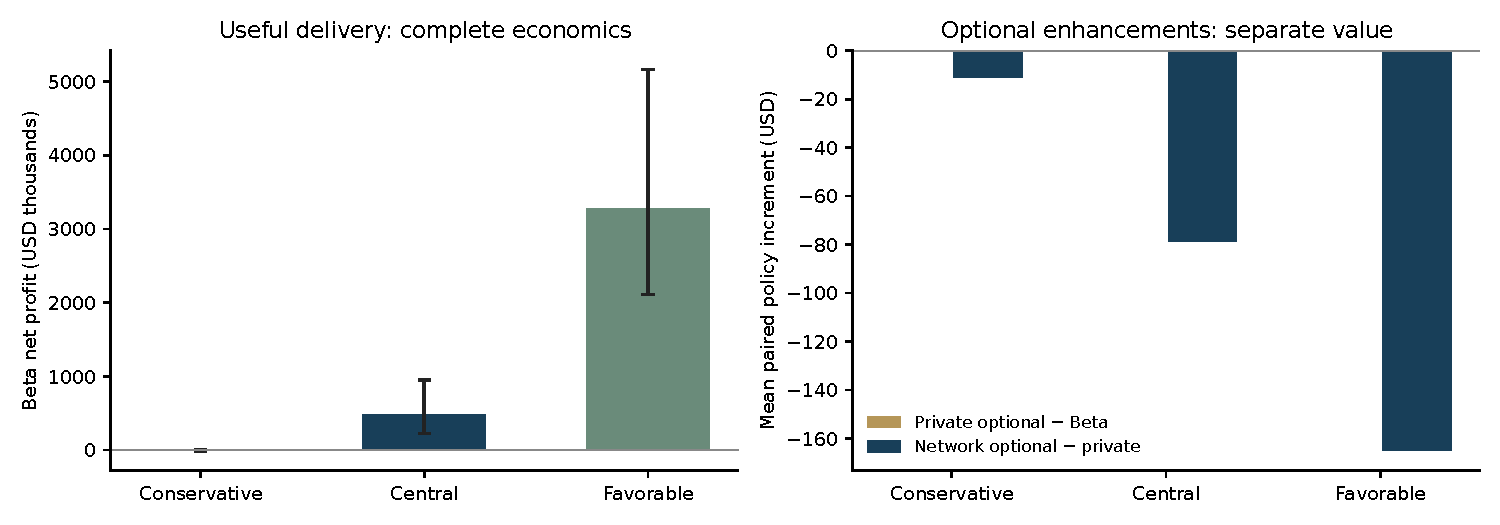
\includegraphics[width=\linewidth]{generated/results_overview.pdf}\caption{Commercial core first. Left: Beta complete-profit medians and 5th--95th percentile ranges. Right: paired mean policy increments from optional private capability decisions and network availability. The scales differ deliberately: large service economics and small enhancement effects are distinct questions.}\end{figure}
\subsection{Optional retained Alpha, sharing and investment}
\begin{table}[htbp]\centering\small\begin{tabular}{lrrrrr}
\toprule
Condition & Network $-$ Beta & Network $-$ private & Retain & Admit & Feedback\\\midrule
Conservative & \usd{-11} & \usd{-11} & 0.0\% & 0.00 & 0.0\%\\
Central & \usd{-79} & \usd{-79} & 0.0\% & 0.00 & 0.0\%\\
Favorable & \usd{-165} & \usd{-165} & 0.0\% & 0.00 & 0.0\%\\
\bottomrule\end{tabular}\caption{Optional-policy mean increments and all-world frequencies, kept separate from Beta commercial success. Retain is an additional B-package purchase. Feedback requires an operating-funded package linking useful collected source work to useful fresh recipient work, positive total and quality-adjusted paired value, and no separate C construction campaign. It is descriptive, not a mandatory investment count.}\end{table}
No primary world purchased portable retention or optional separate capability construction. Ordinary source-agent artifacts remain available under Beta; paid candidate scans and nominated candidates do not establish additional Alpha. The tested policy declined the incremental expenditures. Its small negative network effects reflect the cost and incidental resource consequences of searching, not destruction of the profitable commercial core. This is evidence of the tested policy choosing restraint, not proof that every possible retained capability is worthless or that global optimality has been established.

Conservative: network availability changed mean profit by \usd{-11} (Monte Carlo standard error \usd{0.41}; 5th--95th percentile \usd{-27} to \usd{0}). Private optional decisions changed profit by \usd{0}. Paid scans averaged 1.9, nominated candidates 0.3, and upfront B purchases \usd{0}. There were 0.00 useful capability--project reuse pairs; separate capsules can create multiple pairs for one project. The paired policy effect on distinct useful projects was 0.00. Endogenous network pricing changed mean profit by \usd{8,404} relative to the fixed 65\% diagnostic; this comparison includes any induced resource decisions.

Central: network availability changed mean profit by \usd{-79} (Monte Carlo standard error \usd{1.60}; 5th--95th percentile \usd{-148} to \usd{-31}). Private optional decisions changed profit by \usd{0}. Paid scans averaged 20.4, nominated candidates 2.0, and upfront B purchases \usd{0}. There were 0.00 useful capability--project reuse pairs; separate capsules can create multiple pairs for one project. The paired policy effect on distinct useful projects was 0.00. Endogenous network pricing changed mean profit by \usd{161,153} relative to the fixed 65\% diagnostic; this comparison includes any induced resource decisions.

Favorable: network availability changed mean profit by \usd{-165} (Monte Carlo standard error \usd{2.13}; 5th--95th percentile \usd{-250} to \usd{-94}). Private optional decisions changed profit by \usd{0}. Paid scans averaged 53.3, nominated candidates 3.0, and upfront B purchases \usd{0}. There were 0.00 useful capability--project reuse pairs; separate capsules can create multiple pairs for one project. The paired policy effect on distinct useful projects was 0.00. Endogenous network pricing changed mean profit by \usd{176,018} relative to the fixed 65\% diagnostic; this comparison includes any induced resource decisions.
\begin{table}[htbp]\centering\small\begin{tabular}{lrrrrr}
\toprule
Condition & Beta A & Beta B & Beta C* & Network B & Later C\\\midrule
Conservative & \usd{17,569} & \usd{0} & \usd{5,251} & \usd{11} & \usd{0}\\
Central & \usd{50,541} & \usd{0} & \usd{5,251} & \usd{79} & \usd{0}\\
Favorable & \usd{153,833} & \usd{0} & \usd{5,251} & \usd{165} & \usd{0}\\
\bottomrule\end{tabular}\caption{Disjoint complete-cost records, USD means. A includes delivery, within-job learning, qualification, fees and allocated overhead. B includes extra scans, failed candidates, retention and reuse. *C includes initial bounded venture discovery; later optional C campaigns are identified separately. Refunds reverse revenue, and no source-job construction is charged again to B.}\end{table}
The primary confirmation does not supply a population of funded admissions from which to estimate admission precision or realized skill repayment. Directed funded and recovery fixtures verify software/accounting branches only; their forced capital action is not economic-selection evidence. Any actual funded sensitivity path is separately labeled and retains its all-world frequency. Profitable delivery, useful retained Alpha, productive reinvestment and self-acceleration remain different claims.


\subsection{Conditional break-even screens}\begin{table}[htbp]\centering\small\begin{tabular}{lrrrr}
\toprule
Condition & Useful / month & Required purchase & Validation ceiling* & Capacity upper*\\\midrule
Conservative & 0.229 & 38.0\% & \usd{3,068} & 13.4\\
Central & 0.086 & 2.8\% & \usd{9,196} & 22.0\\
Favorable & 0.039 & 0.6\% & \usd{22,016} & 29.1\\
\bottomrule\end{tabular}\caption{Analytic screens at the confirmation mean posted price. *Validation ceiling is per useful outcome at one useful project/month; capacity is purchased project attempts/month before bursts, queues, retention and maintenance. Complete setup, settlement-runoff overhead and qualification are included; all false passes are refunded in this screen. These are conditional thresholds, not demand evidence or service guarantees.}\end{table}
The primary retention options cost \usd{290.05} for R, \usd{307.95} for V, \usd{569.72} for bundle. Their optimistic reconstruction-only reuse requirements are 5.2 for R, 8.3 for V, 6.2 for bundle. The source job is not charged again. Actual repayment requires enough compatible first encounters with recipients after overlap, transfer, access, upkeep, erosion and the capacity consumed by retention.

For an additional retention bill $K$, maximum affordable expenditure at a decision is cleared cash minus protected liabilities, reserves and headroom. The full ledger determines this ceiling before spending. For constant compatible reuse $u$ and per-use incremental value $b_t$, the prospective screen is $\sum_{t=1}^{H}\delta^t(ub_t-m_t)>K$, where $m_t$ includes remaining maintenance and revalidation. Advancing Beta changes $b_t$; a shorter useful lifetime or lower adoption can make waiting optimal even after a profitable source job.


\subsection{Prespecified sensitivity and ablation results}
The 19 frozen conditions each use 200 independent world IDs and four matched policies. The common stress seed is 951352, separate from the primary confirmation seed. Conditions reuse keyed random streams: there are 3,800 case--world evaluations, not that many mutually independent draws. Every condition and all scalar world outcomes are preserved. Compound changes are explicitly exploratory scenarios, declared before confirmation; they are not isolated causal estimates or calibrated demand forecasts.
\begin{table}[htbp]\centering\scriptsize\begin{tabular}{p{.37\linewidth}rrrr}
\toprule
Condition & Beta profit & Network $-$ Beta & Retention & Admission\\\midrule
Human reference USD 4,900 (C) & \usd{80,729} & \usd{-75} & 0.0\% & 0.0\%\\
One opportunity per month & \usd{311,873} & \usd{-17} & 0.0\% & 0.0\%\\
No job-born candidates & \usd{3,366,012} & \usd{0} & 0.0\% & 0.0\%\\
No separate C research & \usd{3,366,012} & \usd{-160} & 0.0\% & 0.0\%\\
Zero incremental Alpha effects & \usd{3,366,012} & \usd{0} & 0.0\% & 0.0\%\\
Nominal cost-only effects (qualified) & \usd{3,366,012} & \usd{-160} & 0.0\% & 0.0\%\\
All recipients already equivalent & \usd{3,374,109} & \usd{-160} & 0.0\% & 0.0\%\\
Ordinary cross-agent reuse is free & \usd{3,371,504} & \usd{-160} & 0.0\% & 0.0\%\\
Static Beta & \usd{3,365,763} & \usd{-160} & 0.0\% & 0.0\%\\
Faster Beta erosion & \usd{3,368,094} & \usd{-160} & 0.0\% & 0.0\%\\
48 recipients; same compute & \usd{3,401,705} & \usd{-176} & 4.5\% & 1.0\%\\
Specialist routing; same compute & \usd{3,366,179} & \usd{-160} & 0.0\% & 0.0\%\\
Concentrated supported schema & \usd{3,379,446} & \usd{25} & 0.0\% & 0.0\%\\
Double validation activities & \usd{3,351,553} & \usd{-4} & 0.0\% & 0.0\%\\
Double retention activities & \usd{3,366,012} & \usd{-160} & 0.0\% & 0.0\%\\
Stronger correlated errors (C) & \usd{340,246} & \usd{-71} & 0.0\% & 0.0\%\\
80\% authorization, two-month lag (C)* & \usd{413,350} & \usd{-78} & 0.0\% & 0.0\%\\
Looser capacity; quality effects retained & \usd{3,365,422} & \usd{-160} & 0.0\% & 0.0\%\\
Joint static-Beta / larger-pool case* & \usd{10,723,148} & \usd{-1,380} & 93.5\% & 44.0\%\\
\bottomrule\end{tabular}\caption{All prespecified stresses, USD means and all-world frequencies. (C) changes the central condition; other rows change the favorable condition. *Compound scenario. Retention is any additional B purchase; admission is any paid-job capsule admitted within the simulation. No frozen sensitivity produces actual capsule reuse or operating-funded useful feedback. These capability results are qualified by the recipient decision bottleneck described below.}\end{table}

\textbf{Redundancy and attribution.} Removing the modeled Alpha effects changes network profit relative to Beta by \usd{0}; making every recipient equivalent yields \usd{-160}. When ordinary cross-agent reuse is itself free and equivalent, the increment is \usd{-160}. These controls test whether the formal sharing layer adds anything beyond capabilities already available. The nominal cost-only case produces \usd{-160}, but a recipient-valuation defect prevents interpreting it as a clean quality-free ablation. Reliability-linked dollar value must not be inferred solely from avoided token costs.

\textbf{The moving frontier and the recipient pool.} Static Beta produces a mean increment of \usd{-160}, versus \usd{-160} under faster erosion. Forty-eight heterogeneous recipients at unchanged aggregate compute produce \usd{-176}; this isolates recipient-pool structure from simply buying more compute. The joint scenario produces \usd{-1,380}, with useful operating-funded feedback in 0.0\% of worlds. It jointly holds Beta static, expands the recipient pool, increases paid-contract arrivals and pays for fourfold reserved capacity/control resources. Its result cannot be attributed to any one of those changes.

\textbf{Commercial failure conditions.} At the USD 4,900 human reference, mean Beta profit is \usd{80,729}; with one monthly opportunity it is \usd{311,873}. Stronger correlated errors leave 20.1\% material errors among approved deliveries and mean Beta profit of \usd{340,246}. Positive accounting profit alone does not establish an acceptable error rate, buyer trust or product fitness.

The frozen identifier \texttt{loose\_capacity\_cost\_only} changes reserved capacity but retains quality effects; it is therefore labeled accordingly in the table. The distinct \texttt{cost\_only\_alpha} case removes the quality increment. No frozen parameters were changed to repair that naming ambiguity. The primary candidate-scan frequency and one-campaign forecast are bounded heuristics; a policy that stops unproductive searching may do better. No global optimum is claimed.

\textbf{What the frozen Alpha result cannot establish.} The 48-recipient, same-compute case purchases retention in 4.5\% of worlds and admits it in 1.0\%; the compound case purchases in 93.5\% and admits in 44.0\%. Neither produces a capsule use. A post-confirmation independent review found that recipient beliefs and admission forecasts are not harmonized. The candidate posterior mean $(2+s)/(4+n)$ has a ceiling of $26/28=0.92857$ after 24 perfect cases, or $18/20=0.90$ after a 16-case reassessment. It is compared with a known favorable Beta component correctness of at least $0.97$. Even at the lowest permitted price and greatest reconstruction saving, the resulting favorable per-use valuation is negative before acquisition costs. Zero uptake is therefore structurally imposed by this conservative trust rule, rather than evidence that every underlying capability lacks incremental value. Admission and capital forecasts can still expect deployment, creating a controller mismatch.

The frozen cost-only ablation also omits the quality-effect multiplier from recipient valuation, so it can charge a perceived quality penalty although the deployed capability has no modeled quality effect. All frozen outcomes and hashes are preserved; this limitation does not alter Beta-only delivery, cash or profit. The positive USD24.78 increment in the concentrated-schema case has no retention purchase or reuse and is an incidental whole-policy resource/cash effect, not evidence of Alpha.

A deterministic replay of the lowest-ID admitted compound world matches all 95 saved scalar and paired fields. It spends USD232.04 on an admitted package, uses it zero times, and loses USD843.61 relative to Beta. This is an admitted-but-unused mechanism diagnostic, not a new trial. The separate directed QA transfer fixture exercises a useful fresh-recipient branch but loses USD450.05 over the whole paired trajectory; its forced action is never commercial-selection evidence. One fresh-sample posterior-coherence diagnostic is declared separately; it changes beliefs, not actual model capability, and cannot replace the frozen primary or stress findings.


\subsection{One exploratory recipient-belief diagnostic}
After the frozen zero-use result was diagnosed, one new protocol was frozen before a single fresh run: 100 matched world IDs, seed 951557, and three arms (300 complete histories). It uses the previously declared compound condition, with static Beta, 48 recipients, greater contract recurrence and paid additional capacity. This is a post-confirmation exploratory belief sensitivity, not replacement confirmation or evidence of a real market.

The treatment preserves the actual task, capability, failure, cost, cash, demand and resource generators. It retains four prior-equivalent cases but centers the prior on declared construction assumptions: $q_0=\pi q_{\rm good}+(1-\pi)0.65$ and $\hat q=(4q_0+s)/(4+n)$. For a paid-job capsule, $\pi$ is declared reconstruction correctness times retention-generalization success; for separate research it is declared build success. No latent source truth or future outcome is available to the controller. This prior is an unmeasured decision assumption, not a capability bonus. The extension also honors the quality-effect multiplier in reuse valuation; it equals one here and cannot cause this treatment difference.
\begin{table}[htbp]\centering\small\begin{tabular}{lrrrr}
\toprule
Arm & Profit $-$ Beta & Admission & Useful reuse & Useful pairs\\\midrule
Frozen Beta & \usd{0.00} & 0.0\% & 0.0\% & 0.00\\
Frozen network & \usd{-1,300.19} & 38.0\% & 0.0\% & 0.00\\
Declared-prior network & \usd{-1,172.65} & 38.0\% & 36.0\% & 1.53\\
\bottomrule\end{tabular}\caption{Fresh exploratory diagnostic. Frequencies use all 100 worlds. Useful pairs are capsule--project pairs, not necessarily distinct projects. Beta mean complete profit is \usd{11,073,182} in this deliberately strong compound condition. All inputs, full ledgers and negative outcomes are retained.}\end{table}
The declared-prior policy produces useful reuse in 36.0\% of worlds, with 1.71 attempted and 1.53 useful capsule--project uses per world. Admission occurs in 38.0\% of worlds. Relative to the frozen network it improves mean profit by \usd{127.54} (median \usd{0}; 5th--95th percentile \usd{0} to \usd{543.53}; minimum \usd{-152.43}). The revised belief opens a previously blocked reuse path; it does not guarantee a worthwhile retention policy.

\textbf{Beta remains the best tested policy.} The declared-prior network loses \usd{1,172.65} on average relative to Beta (Monte Carlo standard error \usd{42.53}; median \usd{-1,180.54}; 5th--95th percentile \usd{-1,894.47} to \usd{-589.85}). It underperforms Beta in every one of the 100 worlds. Quality-adjusted differences are identical. The paired change in distinct useful accepted projects is zero. Mean extra B spending is \usd{1,254.70}, including rejected candidates and upkeep. Useful transfer is therefore demonstrated within this simulation, but total retention-policy repayment and operating-funded profitable feedback remain unsupported. Both network arms also undertake one optional C campaign in one world; its cost remains in total policy profit (mean USD47.68 across all worlds). These contrasts therefore measure whole-policy effects, not the isolated repayment of each capsule.

This single diagnostic separates a software decision bottleneck from economic success: correcting the belief mismatch can enable useful reuse without making the complete enhancement worthwhile. No further policy or parameter tuning followed. The primary Beta result is unchanged, and no volume, graph size, reuse count or profitable source job is relabeled as recursive improvement. The separately frozen files, four directed extension tests and independent 300-history cash/provenance audit accompany the result.


The README gives exact reproduction commands. The frozen primary wrapper is \texttt{sim/confirm\_v3.py}; the sensitivity wrapper is \texttt{sim/run\_stress\_v3.py}. Both preserve independent seeds and check frozen inputs. Every primary history, monthly ledger and activity receipt is retained in compressed JSONL, with all-world CSVs for analysis. Stress outputs preserve every scalar world and policy contrast. Post hoc deterministic reporting of cash and matched prices is \texttt{analysis/commercial\_cash\_summary.py}; it changes no decision. Publication tables come from \texttt{paper/build\_paid\_results.py}, the threshold/sensitivity/lifecycle renderers and \texttt{paper/build.py}. The bilingual HTML opens offline. Historical protocols and negative development findings are preserved with their status; they are not substituted for this confirmation.


\end{document}